% Compile with XeLaTeX (recommended on Overleaf: Menu > Compiler > XeLaTeX)
% Needed so that Yoruba characters such as ẹ and ọ display correctly.

\documentclass[aspectratio=169,11pt]{beamer}

\usepackage{fontspec}
\usepackage{tikz}
\usetikzlibrary{positioning,shapes.geometric,arrows.meta,calc}
\usepackage{booktabs}
\usepackage{array}

% Colours (Yoruba inspired: deep indigo, warm orange, leaf green)
\definecolor{indigo}{HTML}{1F2A5A}
\definecolor{ember}{HTML}{E8742A}
\definecolor{leaf}{HTML}{2E8B57}
\definecolor{sand}{HTML}{FBF6EE}
\definecolor{ink}{HTML}{222222}
\definecolor{mist}{HTML}{E9ECF5}

\setbeamercolor{normal text}{fg=ink,bg=sand}
\setbeamercolor{structure}{fg=indigo}
\setbeamercolor{title}{fg=white}
\setbeamercolor{frametitle}{fg=white,bg=indigo}
\setbeamercolor{block title}{fg=white,bg=indigo}
\setbeamercolor{block body}{fg=ink,bg=mist}
\setbeamercolor{alerted text}{fg=ember}
\setbeamercolor{itemize item}{fg=ember}
\setbeamercolor{itemize subitem}{fg=ember}
\setbeamercolor{enumerate item}{fg=ember}

\setbeamertemplate{navigation symbols}{}
\setbeamertemplate{itemize items}[circle]
\setbeamertemplate{blocks}[rounded][shadow=false]

% Frame title bar
\setbeamertemplate{frametitle}{%
  \vskip-0.2cm
  \begin{tikzpicture}[remember picture,overlay]
    \fill[indigo] (current page.north west) rectangle ([yshift=-1.15cm]current page.north east);
    \fill[ember] ([yshift=-1.15cm]current page.north west) rectangle ([yshift=-1.22cm]current page.north east);
  \end{tikzpicture}%
  \vskip0.05cm
  {\Large\bfseries\color{white}\insertframetitle\par}
  \vskip0.45cm
}

% Footer with slide number
\setbeamertemplate{footline}{%
  \hfill{\scriptsize\color{indigo}\insertframenumber\,/\,\inserttotalframenumber}\hspace{0.4cm}\vskip0.25cm
}

% Handy helpers
\newcommand{\key}[1]{\textcolor{ember}{\textbf{#1}}}
\tikzset{
  box/.style={rounded corners=4pt,draw=indigo,fill=white,thick,align=center,
              minimum height=1.05cm,text width=2.5cm,font=\small},
  hot/.style={box,fill=ember!15,draw=ember},
  cool/.style={box,fill=leaf!15,draw=leaf},
  flow/.style={-{Stealth[length=2.5mm]},thick,draw=indigo}
}

\title{Ìlè Oúnjẹ}
\subtitle{A Retrieval Augmented Chatbot for Learning Yoruba Cuisine}
\author{Final Year Project Defense}
\date{}

\begin{document}

% ======================= TITLE =======================
\begin{frame}[plain]
  
\begin{tikzpicture}[remember picture,overlay]
    \fill[indigo] (current page.south west) rectangle (current page.north east);
    \fill[ember] ([yshift=2.2cm]current page.south west) rectangle ([yshift=2.3cm]current page.south east);
  \end{tikzpicture}
  \centering
  \vspace{1.3cm}
  {\fontsize{38}{44}\selectfont\bfseries\color{white} Ìlè Oúnjẹ\par}
  \vspace{0.4cm}
  {\Large\color{ember} A chatbot that teaches Yoruba cuisine\par}
  \vspace{0.5cm}
  {\normalsize\color{white} Answers you can trust, because every answer comes from a real dish library\par}
  \vspace{1.2cm}
  {\small\color{white!80} Final Year Project Defense\par}
\end{frame}

% ======================= PROBLEM =======================
\begin{frame}{The problem with plain AI models}
  \begin{columns}[T]
    \column{0.55\textwidth}
      \begin{itemize}
        \item A plain LLM answers from \key{what it learned in training}, like a student answering from memory.
        \item It sounds confident, but sometimes it \key{makes things up}.
        \item This is called a \key{hallucination}.
        \item For culture and food, a wrong ingredient or a wrong origin story is a real problem.
      \end{itemize}
    \column{0.42\textwidth}
      \begin{block}{Our goal}
        A chatbot that only says what is \alert{true and verified} about Yoruba dishes, and that shows the dish picture too.
      \end{block}
  \end{columns}
  \vfill
  \begin{block}{Side note: chatbot versus LLM}
    \footnotesize
    A chatbot is the app you talk to. The LLM is the AI engine inside it. On its own, an LLM answers from what it learned in training, so it can guess. Our project adds retrieval, so the LLM answers from \alert{verified Yoruba dish data} instead.
  \end{block}
\end{frame}

% ======================= SOLUTION =======================
\begin{frame}{The idea: an open book exam}
  \begin{columns}[T]
    \column{0.48\textwidth}
      \begin{block}{Plain LLM}
        A student taking an exam \alert{from memory} (its training data). Fluent, but sometimes guesses.
      \end{block}
      \begin{block}{Our chatbot (LLM plus RAG)}
        A student taking an \alert{open book exam}. It first looks up the right page, then writes the answer from that page.
      \end{block}
    \column{0.48\textwidth}
      \centering
      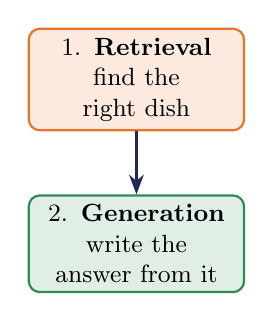
\begin{tikzpicture}
        \node[hot] (a) {1. \textbf{Retrieval}\\find the right dish};
        \node[cool,below=0.8cm of a] (b) {2. \textbf{Generation}\\write the answer from it};
        \path (a) edge[flow] (b);
      \end{tikzpicture}
      \vspace{0.2cm}

      {\small This approach is called \key{RAG}:\\Retrieval Augmented Generation}
  \end{columns}
\end{frame}

% ======================= BIG PICTURE =======================
\begin{frame}{The big picture}
  \centering
  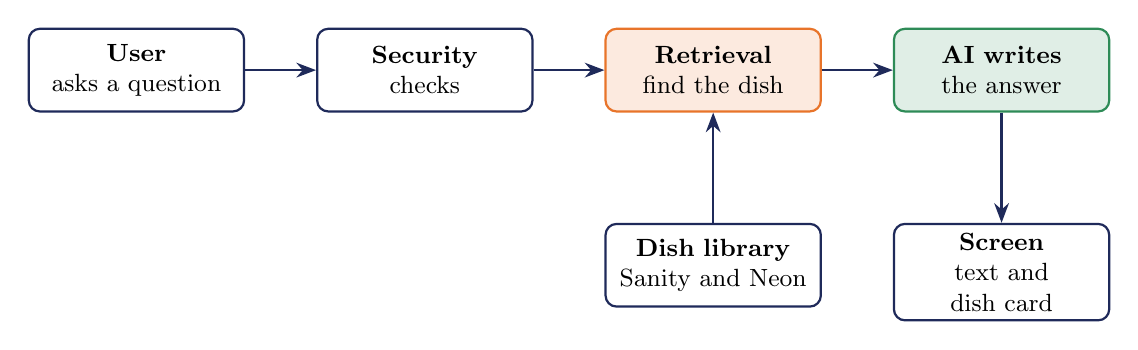
\begin{tikzpicture}[node distance=0.9cm]
    \node[box] (user) {\textbf{User}\\asks a question};
    \node[box,right=of user] (check) {\textbf{Security}\\checks};
    \node[hot,right=of check] (ret) {\textbf{Retrieval}\\find the dish};
    \node[cool,right=of ret] (gen) {\textbf{AI writes}\\the answer};

    \path (user) edge[flow] (check);
    \path (check) edge[flow] (ret);
    \path (ret) edge[flow] (gen);

    \node[box,below=1.4cm of ret] (lib) {\textbf{Dish library}\\Sanity and Neon};
    \path (lib) edge[flow] (ret);

    \node[box,below=1.4cm of gen] (ui) {\textbf{Screen}\\text and dish card};
    \path (gen) edge[flow] (ui);
  \end{tikzpicture}

  \vspace{0.3cm}
  {\small The AI never sees the whole internet. It only sees the dish we found for it.}
\end{frame}

% ======================= STEP 0 =======================
\begin{frame}{Step 0: Preparing the book (done once)}
  \begin{enumerate}
    \item An editor adds dishes in \key{Sanity}, an easy admin page. Each dish has a name, category, picture, background, ingredients with photos, and a recipe.
    \item A script then turns every dish into a list of numbers called an \key{embedding}.
    \item Those numbers are saved in a database (\key{Neon Postgres pgvector}).
  \end{enumerate}
  \vspace{0.2cm}
  \begin{block}{Neon Postgres and pgvector: what is the difference?}
    \small
    \begin{itemize}
      \item \key{Neon Postgres} is the \alert{database}. It stores saved chats and the dish records.
      \item \key{pgvector} is an \alert{extension} that teaches Postgres to store embeddings and search them by meaning.
      \item One line answer: \textit{``pgvector adds vector search to Postgres.''}
      \item Benefit: one database does both jobs, so we did not need a second, separate vector database.
    \end{itemize}
  \end{block}
  \vspace{0.1cm}
  {\small\textcolor{leaf}{\textbf{Why this matters:}} editors can grow the knowledge base without writing any code.}
\end{frame}

% ======================= EMBEDDING =======================
\begin{frame}{What is an embedding?}
  \begin{columns}[T]
    \column{0.52\textwidth}
      \begin{itemize}
        \item A way to turn the \key{meaning} of text into numbers.
        \item Think of it as \key{GPS coordinates for meaning}.
        \item Texts with similar meaning get nearby coordinates.
        \item Model used: Google Gemini \texttt{gemini-embedding-001}, 768 numbers per dish.
      \end{itemize}
    \column{0.45\textwidth}
      \centering
      \begin{tikzpicture}[scale=0.9]
        \draw[thick,draw=indigo!40] (0,0) rectangle (5,4);
        \fill[ember] (1.2,3.0) circle (0.12) node[right,font=\scriptsize] {Àkàrà};
        \fill[ember] (1.8,2.5) circle (0.12) node[right,font=\scriptsize] {fried bean cakes};
        \fill[leaf] (3.6,0.8) circle (0.12) node[above,font=\scriptsize] {Ẹ̀fọ́ rírò};
        \fill[leaf] (3.0,1.3) circle (0.12) node[above left,font=\scriptsize] {vegetable stew};
      \end{tikzpicture}

      {\scriptsize Similar meaning means close together,\\even when the words are different.}
  \end{columns}
\end{frame}

% ======================= JOURNEY =======================
\begin{frame}{The journey of one question}
  \centering
  {\large\itshape ``How do I prepare yam fritters?''}
  \vspace{0.4cm}

  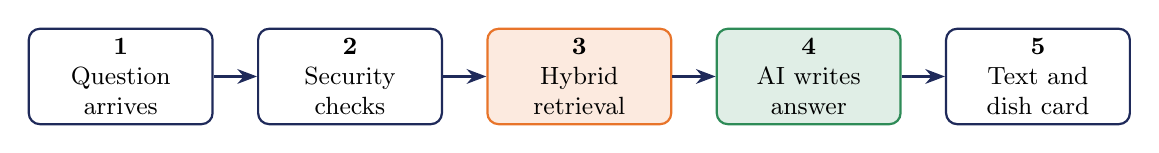
\begin{tikzpicture}[node distance=0.55cm]
    \node[box,text width=2.1cm] (s1) {\textbf{1}\\Question\\arrives};
    \node[box,text width=2.1cm,right=of s1] (s2) {\textbf{2}\\Security\\checks};
    \node[hot,text width=2.1cm,right=of s2] (s3) {\textbf{3}\\Hybrid\\retrieval};
    \node[cool,text width=2.1cm,right=of s3] (s4) {\textbf{4}\\AI writes\\answer};
    \node[box,text width=2.1cm,right=of s4] (s5) {\textbf{5}\\Text and\\dish card};
    \path (s1) edge[flow] (s2);
    \path (s2) edge[flow] (s3);
    \path (s3) edge[flow] (s4);
    \path (s4) edge[flow] (s5);
  \end{tikzpicture}

  \vspace{0.4cm}
  {\small We now go through each step.}
\end{frame}

% ======================= SECURITY =======================
\begin{frame}{Steps 1 and 2: Question and security checks}
  When the message reaches the server, three quick checks happen:
  \vspace{0.2cm}
  \begin{itemize}
    \item \key{Is it a bot?} Bot protection blocks automated abuse.
    \item \key{Is it too many requests?} Rate limits protect cost and the free AI quota.
    \item \key{Is the user signed in?} This decides whether the chat gets saved.
  \end{itemize}
\end{frame}

% ======================= HYBRID =======================
\begin{frame}{Step 3: Hybrid retrieval, two searches at once}
  \begin{columns}[T]
    \column{0.48\textwidth}
      \begin{block}{Keyword search}
        \begin{itemize}
          \item Looks for the user's actual words
          \item Ignores accents, so ``ekuru'' matches ``Èkúrú''
          \item Ignores filler words like ``how'' and ``the''
          \item Dish name matches count the most
        \end{itemize}
        \alert{Strength:} exact names
      \end{block}
    \column{0.48\textwidth}
      \begin{block}{Meaning search}
        \begin{itemize}
          \item Turns the question into an embedding
          \item Finds dishes closest in meaning
          \item Works even when wording is different
        \end{itemize}
        \alert{Strength:} vague questions, such as ``that fried bean snack''
      \end{block}
  \end{columns}
  \vspace{0.2cm}
  \centering {\small Each search produces its own ranked list. Next, we merge the two lists.}
\end{frame}

% ======================= RRF =======================
\begin{frame}{Merging the two lists: Reciprocal Rank Fusion}
  \begin{columns}[T]
    \column{0.5\textwidth}
      Think of \key{two judges} scoring a contest.
      \begin{itemize}
        \item A dish ranked high by \alert{both} judges wins.
        \item A dish ranked high by only one judge can still place well.
        \item One judge alone cannot dominate.
      \end{itemize}
      \vspace{0.2cm}
      {\small The next slides show the exact calculation with real numbers.}
    \column{0.47\textwidth}
      \begin{block}{The formula}
        \centering
        \Large $\displaystyle \text{score} = \sum \frac{1}{60 + \text{rank}}$

        \vspace{0.2cm}
        \footnotesize
        For each list a dish appears in, take $\dfrac{1}{60 + \text{its rank}}$. Then add the results together.
      \end{block}
      \begin{itemize}\small
        \item Rank 1 is the best place, rank 2 is second, and so on.
        \item A dish missing from a list simply earns nothing from it.
      \end{itemize}
  \end{columns}
\end{frame}

% ======================= RRF WORKED EXAMPLE =======================
\begin{frame}{RRF worked example: step 1, the two ranked lists}
  \centering
  User asks: \textit{``that fried bean snack''}
  \vspace{0.3cm}

  \begin{columns}[T]
    \column{0.47\textwidth}
      \begin{block}{Keyword list}
        \small
        \begin{tabular}{@{}cl@{}}
          1st & Ojojo \\
          2nd & Àkàrà \\
          3rd & Mọ́í mọ́í \\
        \end{tabular}

        \footnotesize The word ``fried'' appears most in Ojojo's text.
      \end{block}
    \column{0.47\textwidth}
      \begin{block}{Meaning list}
        \small
        \begin{tabular}{@{}cl@{}}
          1st & Àkàrà \\
          2nd & Mọ́í mọ́í \\
          3rd & Ẹ̀kọ \\
          5th & Ojojo \\
        \end{tabular}

        \footnotesize The meaning ``fried bean cake'' is closest to Àkàrà.
      \end{block}
  \end{columns}

  \vspace{0.2cm}
  {\small Notice the two judges disagree: keyword search puts Ojojo first, meaning search puts Àkàrà first.}
\end{frame}

\begin{frame}{RRF worked example: step 2, the calculation}
  \centering\footnotesize
  \renewcommand{\arraystretch}{1.35}
  \begin{tabular}{@{}lcccccc@{}}
    \toprule
    Dish & Keyword rank & Meaning rank & Keyword points & Meaning points & \textbf{Total} \\
    \midrule
    Àkàrà & 2 & 1 & $\frac{1}{62} = 0.01613$ & $\frac{1}{61} = 0.01639$ & \alert{\textbf{0.03252}} \\
    Mọ́í mọ́í & 3 & 2 & $\frac{1}{63} = 0.01587$ & $\frac{1}{62} = 0.01613$ & 0.03200 \\
    Ojojo & 1 & 5 & $\frac{1}{61} = 0.01639$ & $\frac{1}{65} = 0.01538$ & 0.03178 \\
    Ẹ̀kọ & none & 3 & 0 & $\frac{1}{63} = 0.01587$ & 0.01587 \\
    \bottomrule
  \end{tabular}

  \vspace{0.4cm}
  \begin{block}{Worked line, for Àkàrà}
    \small Keyword rank 2 gives $\frac{1}{60+2}$. Meaning rank 1 gives $\frac{1}{60+1}$. Add them: $0.01613 + 0.01639 = 0.03252$.
  \end{block}
\end{frame}

\begin{frame}{RRF worked example: step 3, the winner rises to the top}
  \begin{columns}[T]
    \column{0.58\textwidth}
      \centering
      \begin{tikzpicture}
        \node[anchor=east,font=\footnotesize] at (0,2.7) {1. Àkàrà};
        \node[anchor=east,font=\footnotesize] at (0,1.9) {2. Mọ́í mọ́í};
        \node[anchor=east,font=\footnotesize] at (0,1.1) {3. Ojojo};
        \node[anchor=east,font=\footnotesize] at (0,0.3) {4. Ẹ̀kọ};
        \fill[ember] (0.1,2.5) rectangle (4.4,2.9);
        \fill[indigo!70] (0.1,1.7) rectangle (4.33,2.1);
        \fill[indigo!70] (0.1,0.9) rectangle (4.30,1.3);
        \fill[leaf!70] (0.1,0.1) rectangle (2.15,0.5);
        \node[font=\scriptsize,anchor=west] at (4.5,2.7) {0.03252};
        \node[font=\scriptsize,anchor=west] at (4.5,1.9) {0.03200};
        \node[font=\scriptsize,anchor=west] at (4.5,1.1) {0.03178};
        \node[font=\scriptsize,anchor=west] at (2.3,0.3) {0.01587};
        \draw[dashed,draw=ember,thick] (-1.6,2.3) rectangle (6.3,3.1);
        \node[font=\tiny,text=ember,anchor=south east] at (6.3,3.1) {kept when we need 1 dish};
      \end{tikzpicture}
    \column{0.4\textwidth}
      \begin{itemize}\small
        \item The \key{top score} becomes the answer.
        \item Àkàrà wins because \alert{both} judges rated it highly.
        \item Ojojo was first on keywords but weak on meaning, so it drops to third.
        \item Ẹ̀kọ appeared in only one list, so its score is about half.
      \end{itemize}
  \end{columns}
\end{frame}

\begin{frame}{How the best candidates are pushed to the top}
  \begin{enumerate}
    \item \key{Collect candidates.} Each search returns a deeper list than needed, at least 10 dishes, so the two lists overlap.
    \item \key{Score every dish} with $\frac{1}{60 + \text{rank}}$ from each list, then add.
    \item \key{Sort by total.} Dishes that appear in \alert{both} lists collect two payments, so they rise above dishes found by only one search.
    \item \key{Keep the top few.} One dish for a specific question, up to five for a ``list'' question.
  \end{enumerate}
  \vspace{0.2cm}
  \begin{block}{Why the number 60?}
    \small It is the standard value from the original RRF research. It keeps the gap between 1st and 2nd place small, so one search alone cannot overrule the other. Equal scores in a list share the same rank, so ties do not create fake precision.
  \end{block}
\end{frame}

% ======================= WHY HYBRID =======================
\begin{frame}{Why use both searches?}
  \begin{columns}[T]
    \column{0.48\textwidth}
      \begin{block}{Keyword alone fails when}
        The user words things differently from the dish text.
      \end{block}
    \column{0.48\textwidth}
      \begin{block}{Meaning alone fails when}
        The user types an exact dish name that must match precisely.
      \end{block}
  \end{columns}
  \vspace{0.4cm}
  \centering
  \Large Together, they cover \key{both} cases.
  \vspace{0.3cm}

  \normalsize
  \textcolor{leaf}{\textbf{Safety net:}} if the meaning search is ever down, the system still works using keyword search alone.
\end{frame}

% ======================= GENERATION =======================
\begin{frame}{Step 4: The AI writes the answer}
  The full text of the found dish is placed into the AI's instructions, with strict rules:
  \vspace{0.2cm}
  \begin{itemize}
    \item Answer \key{only} from this information.
    \item Never invent dishes, ingredients or steps.
    \item If the information is missing, \key{say so} instead of guessing.
    \item Match the answer to the question:
  \end{itemize}
  \vspace{0.1cm}
  \centering\small
  \begin{tabular}{@{}ll@{}}
    \toprule
    User asks & Answer contains \\
    \midrule
    ``What is X?'' & A short definition \\
    ``How do I make X?'' & The steps only \\
    ``List the ingredients'' & The ingredient list only \\
    ``Tell me about X'' & The full description \\
    \bottomrule
  \end{tabular}
\end{frame}

% ======================= OUTPUT =======================
\begin{frame}{Step 5: What the user sees}
  \begin{columns}[T]
    \column{0.5\textwidth}
      \begin{itemize}
        \item The answer \key{streams in word by word}, like someone typing.
        \item Below the text, a \key{dish card} appears.
        \item The card shows the main picture and a scrollable strip of ingredient photos.
        \item A question about one dish shows one card. A list question shows several.
      \end{itemize}
    \column{0.47\textwidth}
      \centering
      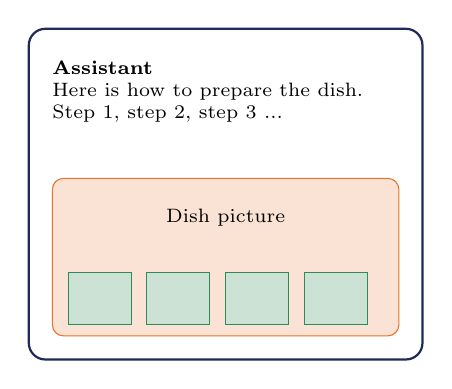
\begin{tikzpicture}
        \draw[rounded corners=6pt,thick,draw=indigo,fill=white] (0,0) rectangle (5,4.2);
        \node[font=\scriptsize,text width=4.4cm,align=left] at (2.5,3.4) {\textbf{Assistant}\\Here is how to prepare the dish. Step 1, step 2, step 3 ...};
        \draw[rounded corners=4pt,fill=ember!20,draw=ember] (0.3,0.3) rectangle (4.7,2.3);
        \node[font=\scriptsize] at (2.5,1.8) {Dish picture};
        \foreach \x in {0.5,1.5,2.5,3.5} {
          \draw[fill=leaf!25,draw=leaf] (\x,0.45) rectangle (\x+0.8,1.1);
        }
      \end{tikzpicture}
  \end{columns}
\end{frame}

% ======================= AUTH =======================
\begin{frame}{Authentication}
  Login is handled by \key{Clerk}, a trusted login service. The project never stores passwords itself.
  \vspace{0.3cm}
  \begin{columns}[T]
    \column{0.48\textwidth}
      \begin{block}{Not signed in}
        \begin{itemize}
          \item Chat immediately
          \item Nothing is saved
          \item Close the tab and it is gone
        \end{itemize}
      \end{block}
    \column{0.48\textwidth}
      \begin{block}{Signed in}
        \begin{itemize}
          \item Chats are saved
          \item History, rename, delete
          \item Only the owner can open or delete a chat
        \end{itemize}
      \end{block}
  \end{columns}
  \vspace{0.2cm}
  \centering {\small Low friction for visitors. Accounts matter only for people who want history.}
\end{frame}

% ======================= PROTECTION =======================
\begin{frame}{Protection and fairness}
  \begin{itemize}
    \item \key{Bot protection} (Vercel BotID) blocks automated abuse.
    \item \key{Rate limits:} 10 messages per hour for signed in users, plus a per IP limit in production.
    \item \key{Why:} to control cost and stop the free AI quota from being drained.
    \item \key{Friendly errors:} if the AI is busy, the system retries automatically and shows a clear message instead of failing silently.
  \end{itemize}
\end{frame}

% ======================= TECH STACK =======================
\begin{frame}{The parts, one line each}
  \centering\small
  \renewcommand{\arraystretch}{1.25}
  \begin{tabular}{@{}>{\bfseries\color{indigo}}p{3.6cm}p{7.2cm}@{}}
    \toprule
    Next.js & The framework the website and server are built with \\
    Sanity & The dish library that editors manage \\
    Gemini & Google's AI, for writing answers and creating embeddings \\
    Neon Postgres and pgvector & The database for saved chats and dish embeddings \\
    Clerk & Login and accounts \\
    Vercel & Where the app is hosted \\
    \bottomrule
  \end{tabular}
\end{frame}

% ======================= DEMO =======================
\begin{frame}{Live demo plan}
  \begin{enumerate}
    \item Ask about a dish by name. Show the answer and the dish card.
    \item Ask with different wording, such as \textit{``that fried bean snack''}. Show that \key{meaning search} still finds the right dish.
    \item Ask for a list, such as \textit{``what soups do you have?''} Show several cards.
    \item Ask about something not in the library. Show that it says \key{``I don't have that dish yet''} instead of inventing an answer.
  \end{enumerate}
\end{frame}

% ======================= LIMITATIONS =======================
\begin{frame}{Limitations and future work}
  \begin{columns}[T]
    \column{0.5\textwidth}
      \textbf{\color{indigo}Limitations}
      \begin{itemize}
        \item It only knows the dishes that were added.
        \item It runs on a free AI quota, so heavy use can be slowed.
        \item After adding dishes, the embedding script must be re-run for meaning search.
        \item It is only as correct as the content put in.
      \end{itemize}
    \column{0.47\textwidth}
      \textbf{\color{indigo}Future work}
      \begin{itemize}
        \item Add many more dishes and regions
        \item Voice questions and Yoruba language input
        \item Automatic re-indexing when content changes
        \item Wider testing with real users
      \end{itemize}
  \end{columns}
\end{frame}

% ======================= Q AND A PREP =======================
\begin{frame}{Questions we expect}
  \begin{block}{Why not just use ChatGPT?}
    General chatbots can invent plausible but wrong food facts. Ours is restricted to verified content that editors control.
  \end{block}
  \begin{block}{How do you stop the AI from lying?}
    It only receives the retrieved dish data, and its instructions forbid inventing anything.
  \end{block}
  \begin{block}{What if the meaning search is down?}
    The system falls back to keyword search, so the chatbot keeps working.
  \end{block}
\end{frame}

% ======================= GLOSSARY =======================
\begin{frame}{Words to remember}
  \small
  \renewcommand{\arraystretch}{1.3}
  \begin{tabular}{@{}>{\bfseries\color{ember}}p{3.8cm}p{7.2cm}@{}}
    RAG & Look up the information first, then answer from it \\
    Embedding & Meaning turned into numbers \\
    Hybrid retrieval & Keyword search and meaning search together \\
    Reciprocal Rank Fusion & The method that merges the two ranked lists \\
    Hallucination & When an AI confidently makes something up \\
    Streaming & The answer appears gradually, not all at once \\
    \bottomrule
  \end{tabular}
\end{frame}

% ======================= SUMMARY =======================
\begin{frame}{Summary}
  \begin{enumerate}
    \item Plain LLMs can \alert{hallucinate}.
    \item We built a \key{RAG} chatbot: find the dish first, then answer from it.
    \item \key{Hybrid retrieval} combines keyword and meaning search for better results.
    \item \key{Clerk} gives optional accounts and saved history.
    \item Result: trustworthy, picture rich answers about Yoruba cuisine.
  \end{enumerate}
\end{frame}

% ======================= THANK YOU =======================
\begin{frame}[plain]
  
\begin{tikzpicture}[remember picture,overlay]
    \fill[indigo] (current page.south west) rectangle (current page.north east);
    \fill[ember] ([yshift=2.2cm]current page.south west) rectangle ([yshift=2.3cm]current page.south east);
  \end{tikzpicture}
  \centering
  \vspace{2.2cm}
  {\fontsize{36}{42}\selectfont\bfseries\color{white} Ẹ ṣé!\par}
  \vspace{0.3cm}
  {\Large\color{ember} Thank you. Questions?\par}
\end{frame}

\end{document}
